\documentclass[openany]{book}
\usepackage{a4wide}
\usepackage[utf8]{inputenc}

\renewcommand{\chaptername}{Kapitola}

%\usepackage{amsmath}
%\usepackage{amsfonts}
%\usepackage{amssymb}
%\usepackage{amsthm}
\usepackage{hyperref}
%\usepackage[slovak]{babel}
\usepackage[T1]{fontenc}

\usepackage{rotating}

\usepackage{pdfpages}

\DeclareUnicodeCharacter{00A0}{~}

\title{Ako sa brániť proti polícii a iným orgánom pri ich neoprávnených zásahoch\footnote{pracovná verzia 4bc0dca0a53db0813f90dc735446681a}}

\author{Michal Mal\'{y}\\
\texttt{m.m.maly@gmail.com}
}

\date{10. Apríl 2011}

%\titlerunning{Ako sa brániť proti polícii a iným orgánom pri ich neoprávnených zásahoch}
%\authorrunning{Michal Malý}

\def\eps{\varepsilon}

\newcommand{\zakon}[1]{\href{http://jaspi.justice.gov.sk/jaspiw1/index_jaspi0.asp?MOD=html&FIR=demo&JEL=n&AGE=zak&IDC=#1}{#1}}
\newcommand{\vznp}{v znení neskorších predpisov}

\begin{document}

\maketitle

\chapter*{Úvod}

Táto publikácia nemá navádzať  na nezákonné konanie. Ma poskytnúť čitateľovi -- občanovi -- prehľad práv, ktoré ho chránia pred svojvoľnými, neoprávnenými, či nevhodnými zásahmi polície alebo iných orgánov štátnej či súkromnej moci, a tiež prehľad predpisov, ktorými sa majú riadiť, a povinností, ktoré od nich možno vyžadovať.

Bezpečnostné zložky, akými sú polícia alebo súkromné bezpečnostné služby, majú za úlohu chrániť oprávnené záujmy. Mohlo by sa zdať, že potrebujú silné právomoci, aby poriadok mohli efektívne chrániť. Avšak proti tomuto záujmu vždy stojí možnosť zneužitia ich právomoci, hrozba policajného štátu. Postavenie slabého občana proti týmto organizovaným zložkám je vždy nerovné. Preto je dobrým zvykom, že na vyváženie nerovnosti majú tieto zložky rôzne povinnosti, ktoré musia starostlivo dodržiavať, aby sa zabránilo zneužitiu moci a zároveň sa zvýšila kontrola nad ich konaním zo strany verejnosti.

Príkladom takejto povinnosti je nosenie menovky: občan povinnosť menovku nosiť nemá \footnote{Našťastie! :-) Alebo...zatiaľ?}, ale policajt či sbs-kár takúto povinnosť má. 

Tato publikácia môže zároveň slúžiť  pre príslušníkov týchto zložiek. Ak majú záujem budovať  svoj dobrý vzťah k verejnosti, mali by poznať svoje povinnosti a pochopiť, prečo sú v niektorých povinnostiach ,,znevýhodnení'' voči tým, proti ktorým zasahujú.

\chapter{Niekoľko dôležitých upozornení}

\begin{itemize}
\item Aj policajti sú ľudia. Nechcú Vám  (vždy:-]) zle, a teda je prehnané považovať ich automaticky za nepriateľov a zaujať formálny, nepriateľský postoj. 

\item Aj policajti sú ľudia. Robia chyby, ako každý. Chcú vykonávať svoju prácu. Skúste sa vžiť  do ich situácie a predstaviť si, ako by ste ju riešili vy.
 
\item Buďte vždy slušní, hoci budete aj asertívni. Nenechajte sa vyprovokovať k nadávkam, či nebodaj násiliu. Môže Vám to veľmi uškodiť a situáciu zhoršiť.

\item Riešiť situáciu formálne, odvolávaním sa na zákony, nemusí byť vždy najlepšie riešenie. Napríklad v policajtovi, ktorý by Vám  dal inak malú pokutu, môže váš prístup vzbudiť dojem chytráckosti, a rozhodne sa Vám dať vyššiu pokutu. Ale možná je aj opačná situácia: ak policajt zistí, že viete, o čom hovoríte, nechá Vás na pokoji.
\end{itemize}

\chapter{Vedeli ste, že...}

Nasledovné odseky uvádzame vo vzťahu k Polícii SR, obdobne sa však vzťahujú aj na mestskú políciu, železničnú políciu, a podobne. Podrobnosti o rozdieloch medzi nimi si vysvetlíme bližšie v ďalšej kapitole.

\section*{...nemáte povinnosť nosiť občiansky preukaz?}

Povráva sa, že občiansky preukaz treba nosiť všade so sebou. Nemožno tvrdiť, že to nie je praktická rada -- človek môže zrazu chcieť niečo neplánovane vybaviť v banke -- ale treba povedať, že povinnosť mať občiansky preukaz stále pri sebe u nás neexistuje. Niekedy ľudia zvyknú dodávať aj: netreba mať do 50 metrov od domu (čísla sa rôznia, asi podľa toho, ako má kto ďaleko smetný kôš:-).

Zákon\footnote{Aktuálne znenie, na ktoré sa budeme aj tu odvolávať, je zákon č. \href{http://jaspi.justice.gov.sk/jaspiw1/index_jaspi0.asp?MOD=html&FIR=demo&JEL=n&AGE=zak&IDC=224/2006}{224/2006} Z. z. o občianskych preukazoch a o zmene a doplnení niektorých zákonov v znení zákonov 693/2006 Z. z., 647/2007 Z. z., 445/2008 Z. z. } takúto povinnosť ale neustanovuje, bez ohľadu na vzdialenosť. Kedysi, ešte za socializmu v rokoch 1953-1958, takúto povinnosť ustanovovalo vládne nariadenie\footnote{Vládne nariadenie 61/1953 Zb. o občianskych preukazoch, v \S 6 Povinnosti občana hovorilo: \\
\begin{quote}
\emph{Občan, ktorý má občiansky preukaz, je povinný: 
\begin{itemize}
\item[] a) neustále nosiť občiansky preukaz a preukazovať sa ním na vyzvanie orgánov na to splnomocnených
(...)
\end{itemize} }
\end{quote}
}. To však už hodných pár rokov neplatí. (Podobný zákon však platí napr. v Srbsku\footnote{Článok 21, Zakon o ličnoj karti (Zákon o občianskych preukazoch).})

Situácia však nie je taká jednoduchá. Treba vysvetliť, čo všetko zákon ustanovuje.

Najprv si povedzme, prečo je občiansky preukaz taký užitočný.
\begin{itemize}

\item vlastní ho každý

\begin{quote}
\emph{Občiansky preukaz je povinný mať každý občan, ktorý dovŕšil pätnásty rok veku a má trvalý pobyt na území Slovenskej republiky, ak tento zákon neustanovuje inak.}
\end{quote}

\item údaje v ňom zapísané sa považujú za preukázané pri predložení

\begin{quote}
\emph{
\textbf{§ 4}
\begin{itemize}
\item[] (1) Údaje v občianskom preukaze v rozsahu ustanovenom v § 3 ods. 1, 2 a 3 písm. c) nahrádzajú verejné listiny o skutočnostiach v rozsahu, ako sú uvedené v občianskom preukaze.
\item[] (2) Pri preukazovaní skutočnosti uvedenej v občianskom preukaze občan nie je povinný predkladať ďalší doklad, ak tento zákon neustanovuje inak.
\end{itemize}
}
\end{quote}


\end{itemize}

To znamená, že ak mám v občianskom preukaze zapísaný titul, môžem túto skutočnosť preukázať občianskym preukazom. Ale nič to už nehovorí o tom, kým a z čoho mi bol titul udelený. Samozrejme, vždy môžem skutočnosti dokladať aj iným spôsobom -- že mám v občianskom preukaze zapísaný titul, neznamená, že nemôžem predložiť diplom. Táto analógia je dôležitá pre pochopenie, že aj totožnosť môžem dokladovať iným spôsobom, ako občianskym preukazom.

Ďalej existuje oprávnenie policajta požadovať preukázanie totožnosti. Dôležité časti znejú takto\footnote{Zákon \href{http://jaspi.justice.gov.sk/jaspiw1/index_jaspi0.asp?MOD=html&FIR=demo&JEL=n&AGE=zak&IDC=171/1993}{171/1993} Z.z. o Policajnom zbore (
Úplné znenia platných zákonov nájde čitateľ na konci knihy.)}:

\begin{quote}
\textbf{§ 18\\
Oprávnenie požadovať preukázanie totožnosti}
\begin{itemize}

\item[] (1) Policajt je oprávnený vyzvať osobu, ak je to potrebné na plnenie úloh podľa tohto zákona, aby preukázala svoju totožnosť dokladom totožnosti9).
\item[] (...)
\item[] (3) Ak vyzvaná osoba odmietne preukázať svoju totožnosť podľa odseku 1 alebo 2, policajt je oprávnený takúto osobu predviesť na útvar Policajného zboru za účelom zistenia jej totožnosti.

\item[] (4) Ak vyzvaná osoba nemôže preukázať svoju totožnosť podľa odseku 1 alebo 2 a ani po predchádzajúcom poskytnutí potrebnej súčinnosti nemôže hodnoverne preukázať svoje meno a priezvisko, dátum narodenia a adresu bydliska, policajt je oprávnený postupovať podľa odseku 3. Hodnovernosť preukázania mena a priezviska, dátumu narodenia a adresy bydliska posudzuje policajt podľa dôvodu zisťovania totožnosti osoby.

\item[] (5) Policajt je povinný odovzdať predvedenú osobu orgánom činným v trestnom konaní, inému príslušnému orgánu alebo príslušnému zariadeniu, ak zistí, že sú dôvody na jej odovzdanie, inak osobu ihneď prepustí.

\item[] (...)
\item[] (6) Ak ide o osobu vyhlásenú za nezvestnú, policajt o jej nájdení vyrozumie toho, kto nezvestnosť tejto osoby oznámil. Ak táto osoba nie je plnoletá, odovzdá ju zákonnému zástupcovi alebo príslušnému orgánu alebo príslušnému zariadeniu; ak ide o osobu pozbavenú spôsobilosti na právne úkony, odovzdá túto osobu jej zákonnému zástupcovi alebo príslušnému zariadeniu, a ak ide o osobu duševne chorú, odovzdá ju príslušnému zariadeniu.

\item[] (7) Ak policajt nezistí totožnosť osoby do 24 hodín od jej predvedenia, je povinný túto osobu prepustiť.

\item[] (8) O predvedení a odovzdaní osoby napíše policajt úradný záznam.
\item[] (...)
\end{itemize}

\end{quote}


Tu treba upozorniť na niekoľko skutočností. Jednak je policajt oprávnený požadovať totožnosť len vtedy, ak je to potrebné na plnenie úloh vyplývajúcich zo zákona. Nemôže teda svojvoľne buzerovať občanov. Koná totiž z pozície štátneho orgánu, a tie \emph{môžu konať iba na základe ústavy, v jej medziach a v rozsahu a spôsobom, ktorý ustanoví zákon}. Na perlustráciu by mal teda mať dôvod. Asi sa dá tušiť, že tento dôvod si policajt môže vymyslieť -- ak to urobí, pozícia občana ostáva rovnaká, hoci sa môže neskôr na postup policajta sťažovať.

Ďalej, policajt musí \emph{poskytnúť potrebnnú súčinnosť}, zákon však nešpecifikuje presne, čo to je. Mohlo by to znamenať, že vás odvezie domov, aby ste mu občiansky ukázali. Čo ak však bývam 100 km ďaleko? Ale totožnosť sa predsa dá doložiť aj inak. Môžete nadiktovať svoje údaje, ktoré si policajt vie overiť v databáze. Možete napr. ukázať kreditnú kartu -- oficiálny doklad to samozrejme nie je, ale niečo to ukazuje, hlavne, ak ju pred ním viete použiť a vybrať peniaze v bankomate. 

V každom prípade, totožnosť neodmietate preukázať, teda zákon ste neporušili, a nemôžete dostať pokutu. Ak sa však toto všetko policajtovi nezdá hodnoverné, môže Vás predviesť, čo môže byť otrava.

Ešte k prelustráciám: Často sa policajti na občiansky preukaz \emph{spýtajú}. Ak im vtedy preukaz ukážete, môžu pri Vašej prípadnej sťažnosti namietať  že neporušili zákon, pretože Vás k tomu nevyzvali. Otázne je, nakoľko by bola taká obrana platná \footnote{Ak si od Vás občiansky preukaz pýta obyčajný človek, nemusíte mu ho ukázať, ale ani on zákon neporušuje -- nie je zakázané  pýtať sa na občiansky preukaz. Policajt však koná ako štátny orgán -- preto môže konať len na základe zákona. Iste je však rozumné predpokladať, že je zároveň aj človek, nemožno jeho výkon zhustiť do zbierky formálnych predpisov.}. Ak si chcete byť istí, že to policajti myslia vážne, a ste odhodlaní sa sťažovať, pretože považujete ich postup za buzeráciu, požiadajte ich, nech použijú príslušnú výzvu\footnote{
\emph{
\textbf{§ 12}
\begin{itemize}
\item[] (1) Policajt je pri vykonávaní služobného zákroku povinný, ak to povaha a okolnosti dovoľujú, použiť výzvu zodpovedajúcu zákroku.
\item[] (2) Ak to povaha služobného zákroku vyžaduje, pred výzvou použije slová ,,V mene zákona''.
\end{itemize}
}}. Vtedy je ich postavenie záväzné a Vaša povinnosť zrejmá.



\section*{...policajt Vás nesmie bezdôvodne prehľadať?}

Predstavte si situáciu, že idete po ulici, a policajti Vás zastavia. Pýtajú občiansky preukaz, pýtajú sa, kam idete, či pri sebe nemáte zbrane alebo drogy. Nazrú Vám do tašiek. Rozmýšľate, čím ste boli podozriví, a či to vlastne môžu ...

Policajti okrem toho, že môžu (pripomíname -- len na plnenie úloh zákona!) vyžadovať preukázanie totožnosti, majú oprávnenie hľadať zbraň:

\begin{quote}
(1) Policajt je oprávnený presvedčiť sa, či osoba, proti ktorej vykonáva služobný zákrok, nemá pri sebe zbraň (§ 14 ods. 5), a ak ju má, odňať ju.
\end{quote}

Toto oprávnenie by teoreticky mohli použiť na prehľadanie osoby. Ani tento úkon však nesmú robiť bezdôvodne, ako o tom rozhodol aj Európsky súd pre ľudské práva v relatívne novom rozsudku z 12. januára 2010, prípad 4158/05 \emph{\href{http://cmiskp.echr.coe.int/tkp197/view.asp?action=html&documentId=860909&portal=hbkm&source=externalbydocnumber}{Gillian and Quinton v. The United Kingdom}}. Kevina Gilliana a Pennie Quinton zastavila polícia v blízkosti demonštrácie. Pána Gilliana, ktorý sa chcel demonštrácie zúčastniť, zastavili na 20 minút, slečna Quinton, novinárka, ktorá prišla natočiť zábery, bola prehľadávaná podľa jej slov asi 30 minút (podľa policajného záznamu 5 minút). Navyše jej zakázali filmovať, napriek tomu, že policajtom ukazovala aj svoj novinársky preukaz. 

Britský zákon v tom čase hovoril, že za určitých podmienok možno zastaviť a prehľadávať osobu bez toho, aby bol potrebný dôvod -- hlavný arument pre takúto úpravu bol, aby sa policajní dôstojníci nebáli prehľadávať osoby, o ktorých majú podozrenie, ale nevedeli by ho dostatočne odôvodniť . Treba poznamenať, že samotný text britského zákona, popis oprávnení policajta, procedúr, ako aj kontrola nad tým, za akých podmienok možno takúto kontrolu vykonať, sú omnoho podrobnejšie, ako je to v porovnaní so slovenským zákonom. Okrem iného má prehľadávaná osoba právo na kópiu záznamu o prehľadaní. Napriek tomu súd rozhodol, že takéto bezdôvodné prehľadávanie bolo porušením Článku 8 Dohovoru o ochrane ľudských práv a základných slobôd\footnote{
\textbf{Článok 8 - Právo na rešpektovanie súkromného a rodinného života}
\begin{enumerate}
\item Každý má právo na rešpektovanie svojho súkromného a rodinného života, obydlia a korešpondencie.
\item Štátny orgán nemôže do výkonu tohto práva zasahovať okrem prípadov, keď je to v súlade so zákonom a nevyhnutné v demokratickej spoločnosti v záujme národnej bezpečnosti, verejnej bezpečnosti, hospodárskeho blahobytu krajiny, predchádzania nepokojom a zločinnosti, ochrany zdravia alebo morálky alebo ochrany práv a slobôd iných. 
\end{enumerate}
}. 

Poznamenajme, že v USA sú takéto prípady ošetrené Štvrtým dodatkom, ktorý zakazuje neodôvodnené prehľadávanie, a bližšie spresnené prípadmi Terry v. Ohio, Michigan v. Long.

%+ pribeh. Navyše iné dôkazy, ktoré by takto našiel (napr. drogy), nesmie proti Vám použiť.

\section*{...policajtovi nemusíte odpovedať na každú otázku?}

Pozastavme sa ešte nad naším príbehom: Polícia sa Vás pýtala, kam idete a podobne. Polícia má, samozrejme, právo požadovať informácie, ktoré sú potrebné na odhalenie priestupku a podobne. Toto sa nazýva \emph{oprávnenie požadovať vysvetlenie}. Netreba však pri pátraní zabúdať na naše ústavné právo odoprieť výpoveď, ak by sme tým mohli poškodiť sebe, alebo blízkej osobe. Na toto pamätá aj príslušné ustanovenie o \emph{oprávnení požadovať vysvetlenie}. Ako sme spomínali v úvode, určité povinnosti musí policajt starostlivo dodržať, pretože je voči občanovi v silnejšej pozícii. V tomto prípade ide o nutnosť poučiť osobu pred podaním vysvetlenia.

\begin{quote}
§ 17 
Oprávnenie požadovať vysvetlenie
\begin{itemize}
\item[] (1) Policajt je oprávnený požadovať potrebné vysvetlenie od osoby, ktorá môže prispieť k objasneniu skutočností dôležitých pre odhalenie priestupku alebo správneho deliktu a na zistenie jeho páchateľa, ako aj na vypátranie hľadaných alebo nezvestných osôb a vecí. V prípade potreby je policajt oprávnený vyzvať osobu, aby sa ihneď alebo v určenom čase dostavila na útvar Policajného zboru na spísanie zápisnice o podaní vysvetlenia alebo, ak ide o objasňovanie priestupku, na spísanie záznamu alebo zápisnice do správy o výsledku objasňovania priestupku. 

\item[] (2) Ak osoba bez dostatočného ospravedlnenia alebo bez závažných dôvodov výzve podľa odseku 1 nevyhovie, môže ju policajt predviesť na útvar Policajného zboru za účelom podania vysvetlenia. O predvedení spíše policajt úradný záznam. 

\item[] (3) Zápisnica o podaní vysvetlenia musí byť s osobou spísaná ihneď po jej predvedení. 

\item[] (4) Vysvetlenie môže odmietnuť iba osoba, ktorá by ním sebe alebo blízkej osobe8) spôsobila nebezpečenstvo trestného stíhania, a ak ide o priestupok, nebezpečenstvo postihu za priestupok alebo osoba, ktorá by ním porušila spovedné tajomstvo alebo tajomstvo informácie, ktorá jej bola zverená ústne alebo písomne pod podmienkou mlčanlivosti ako osobe poverenej pastoračnou starostlivosťou. 

\item[] (5) Vysvetlenie sa nesmie požadovať od osoby, ktorá upozornila, že by ním porušila zákonom uloženú alebo uznanú povinnosť mlčanlivosti, a nebola od tejto povinnosti oslobodená. 

\item[] (6) Policajt je povinný poučiť osobu o možnosti odmietnuť vysvetlenie podľa odsekov 4 a 5. 

\item[] (7) Policajt je povinný predvedenú osobu odovzdať orgánom činným v trestnom konaní alebo inému príslušnému orgánu, ak zistí, že sú dôvody na jej odovzdanie, inak musí osobu ihneď prepustiť, čo vyznačí v úradnom zázname o predvedení. 

\item[] (8) Kto sa na výzvu podľa odseku 1 dostaví, má nárok na náhradu nutných výdavkov a na náhradu ušlého zárobku (ďalej len "náhrada"). Náhradu poskytuje Policajný zbor. Nárok na náhradu nemá ten, kto sa dostavil len vo vlastnom záujme alebo pre svoje protiprávne konanie. 

\item[] (9) Nárok na náhradu podľa odseku 8 zaniká, ak ho oprávnená osoba neuplatní do ôsmich dní odo dňa, keď sa na výzvu podľa odseku 1 dostavila; oprávnenú osobu o tom treba poučiť. 
\end{itemize}
\end{quote}

Čiže ako vidíme, ak sa policajt na niečo opýta, musí Vás zároveň aj poučiť o možnosti odoprieť podať vysvetlenie. Ak tak neurobí, sám porušuje zákon. V takom prípade na otázku nereagujte (veď sa vlastne pýtal ,,len tak, medzi rečou''). Ak bude policajt naliehať, požadujte o zaprotokolovanie skutočnosti, že Vás pred podaním vysvetlenia nepoučil.

Dodáme, že napr. v USA je ustanovená\footnote{tzv. Miranda rights, podľa prípadu Miranda v. Arizona 384 U.S. 436 (1966)}  povinnosť poučiť osobu o práve mlčať a spýtať sa, či svojim právam rozumie. Ak tak neurobí, nemožno jej výroky proti nej použiť. Určite to poznáte z filmov. :-)


%MIRANDA?

\section*{...policajtov si môžete fotografovať, kamerovať a nahrávať bez ich súhlasu?}

Každý požíva právo na ochranu svojej osoby, ako hovorí Občiansky zákonník\footnote{Zákon č. \href{http://jaspi.justice.gov.sk/jaspiw1/index_jaspi0.asp?MOD=html&FIR=demo&JEL=n&AGE=zak&IDC=40/1964}{40/1964} Zb. Občiansky zákonník v znení neskorších predpisov}: 

\begin{quote}
\textbf{Ochrana osobnosti\\
§ 11}

Fyzická osoba má právo na ochranu svojej osobnosti, najmä života a zdravia, občianskej cti a ľudskej dôstojnosti, ako aj súkromia, svojho mena a prejavov osobnej povahy.

\textbf{§ 12}
\begin{itemize}
\item[] (1) Písomnosti osobnej povahy, podobizne, obrazové snímky a obrazové a zvukové záznamy týkajúce sa fyzickej osoby alebo jej prejavov osobnej povahy sa smú vyhotoviť alebo použiť len s jej privolením.

\item (2) Privolenie nie je potrebné, ak sa použijú písomnosti osobnej povahy, podobizne, obrazové snímky alebo obrazové a zvukové záznamy na úradné účely na základe zákona.

\item (3) Podobizne, obrazové snímky a obrazové a zvukové záznamy sa môžu bez privolenia fyzickej osoby vyhotoviť alebo použiť primeraným spôsobom tiež na vedecké a umelecké účely a pre tlačové, filmové, rozhlasové a televízne spravodajstvo. Ani také použitie však nesmie byť v rozpore s oprávnenými záujmami fyzickej osoby.
\end{itemize}
\end{quote}

Na fotografovanie osôb musíte teda vo všeobecnosti mať ich povolenie, okrem televízie a tak podobne. 

Avšak pri verejných činiteľoch je to iné. Samotný Ústavný súd rozhodol\footnote{\href{http://www.concourt.sk/Zbierka/2001/10_01s.pdf}{Nález Ústavného súdu Slovenskej republiky II. ÚS 44/00}}, že \emph{u osôb verejného záujmu dochádza k zúženiu priestoru ich súkromnej sféry, v dôsledku čoho sa primerane znižuje aj úroveň ochrany ich osobnostných práv} a ďalej, \emph{výkon zákonnej právomoci verejného činiteľa (...) nebolo možné považovať za prejav jeho osobnej povahy a ani za súčasť jeho základného práva na súkromie}. 

Policajta, ako aj iné verejne činné osoby, si teda môžete pri výkone ich práce fotografovať, kamerovať, či nahrávať aj bez ich súhlasu. Takýto záznam môže poslúžiť aj ako vhodný dôkaz korupčného, či inak nevhodného správania. 

\section*{...polícia Vás môže odpočúvať, a nikdy sa o tom nedozviete?}

Áno, je to tak. Polícia má právo na základe rozhodnutia súdu odpočúvať osoby, na základe podozrenia. Samozrejme, odpočúvaná osoba o tom nie je upovedomená ;), a to ani po skončení vyšetrovania, ani ak bola nevinná. Často to človek zistí len dodatočne, zo spisov v konaní proti nemu alebo proti osobe jemu známej. Keďže nad odpočúvaním neexistuje verejná kontrola, bolo by namieste, aby dohľad nad vykonávaním odposluchov bol dostatočný. Vieme však, že aj tam, kde verejná kontrola existuje, dochádza k prešľapom.

Typické býva, že polícia ani poriadne neodôvodní, prečo by osoba mala byť odpočúvaná, a súd to schváli. Napríklad manželku môžu odpočúvať preto, že to ,,je potrebné pre objasnenie trestnej činnosti jej manžela'' a ,,získanie informácií je iným spôsobom neúčinné, resp. podstatne sťažené''. Takéto a podobné prípady môžu skončiť na Ústavnom súde a byť ,,ocenené'' peknou sumičkou 450 000 Sk\footnote{Nález Ústavného súdu Slovenskej republiky \href{http://www.concourt.sk/Zbierka/2008/08_30s.pdf}{sp. zn. III. ÚS 80/08 z 27. mája 2008}, nález sp. zn. \href{http://www.concourt.sk/Zbierka/2006/06_31s.pdf}{I. ÚS 274/05}}. 


Odporučíme však nespoliehať sa na Ústavný súd, ale brániť sa, ako človek vie -- technológiou: Dnes už sú aj zadarmo prístupné programy, ktoré bezpečne šifrujú emaily\footnote{GNU Privacy Guard (skratka GnuPG alebo GPG), \url{www.gnupg.org}, existujú aj pluginy do rôznych obľúbených emailových klientov, napr. \href{http://enigmail.mozdev.org}{Enigmail} pre Thunderbird }, dáta na počítači\footnote{TrueCrypt, \url{www.truecrypt.org}}, alebo aj chatovanie cez instant messaging\footnote{Pre ICQ existujú rôzne pluginy. Protokol XMPP (Jabber) je na tom ešte lepšie, možnosť kryptovania je priamo súčasťou špecifikácie a mnohé Jabber servery ho poskytujú. }. O tejto problematike v prípade záujmu nájde človek mnohé a aktuálne informácie na internete, napr. \cite{root}.

Do telefónu háklivé veci rozumný človek radšej nebude rozoberať.


\section*{...policajná hliadka sa na svedectve proti Vám nemôže ,,dohodnúť'' ?}

Stane sa, že správanie vodiča polícia bezdôvodne označí za priestupok. Vodičovi chcú napríklad ,,našiť'' jazdu na červenú alebo nezastavenie na stopke\cite{lejkova}. Vodič sa cíti nevinný, policajti si tvrdia svoje. Sú dvaja a tvária sa, že v prípade potreby ľahko dosvedčia vodičovu vinu. Dve svedectvá proti jednému, vodič bezmocne radšej zaplatí pokutu.

No nie je to tak\footnote{Za nasmerovanie v tomto prípade ďakujem diskutujúcemu ,,Živel'' v diskusii pod spomínaným článkom.}. Najvyšší súd rozhodol v podobnom prípade (vodič si údajne nezapol bezpečnostný pás), že \emph {správne orgány nemôžu pri tomto type priestupku vychádzať len z
tvrdení policajnej hliadky, ak o spáchaní priestupku žalobcom neexistujú žiadne iné dôkazy, než jej hlásenie o spáchaní priestupku, ak osoba obvinená zo spáchania priestupku tvrdí opak. Je úlohou policajnej hliadky zabezpečiť dostatok dôkazov, ktoré by neskoršie tvrdenia osoby obvinenej z priestupku, že priestupok nespáchala, mohli
byť vyvrátené. Napríklad fotodokumentáciou.}\footnote{\href{http://www.supcourt.gov.sk/data/att/2074\_subor.pdf}{Rozhodnutie Najvyššieho súdu SR 8Sžo/173/2010}}

Napriek drobnej gramatickej chybe vo formulácii preto tvrdíme -- smelo!

Treba tiež poznamenať, že ak vodič daný priestupok skutočne nespáchal, nepravidvá výpoveď policajtov by bola minimálne priestupkom podľa § 21 ods. 1 písm. f), v prípade, že by sa vodič odvolal a pojednávalo by sa pred súdom, už i trestným činom podľa § 346 Trestného zákona. Pre korektnosť treba poznamenať, že tieto postihy hrozia i vodičovi, ak by klamal.

Ďalej, ak by policajti úmyselne klamali napríklad preto, aby nazbierali viac ,,bodov'' za odhalené priestupky, alebo jednoducho v úmysle uškodiť vodičovi, páchali by i trestý čin zneužívania právomoci verejného činiteľa (§ 326 TZ).

\chapter{Kto môže použiť donucovacie prostriedky?}

Zákon umožňuje príslušníkom niektorých orgánov, aby v prípade potreby použili násilie na ochranu oprávnených záujmov. Násilie môže spočívať v použití hmatov, chvatov, úderov, kopov sebaobrany alebo aj v použití zbraní, pút, zvieraťa a ďalších donucovacích prostriedkov. Rozsah prostriedkov, ktoré môžu orgány použiť, ich oprávnenia a účel, za ktorým môžu zasahovať, sú rôzne. 

Každý pozná armádu\footnote{Zákon \zakon{321/2002} Z.z. o ozbrojených silách Slovenskej republiky \vznp}, políciu\footnote{Zákon \zakon{171/1993} Z.z. o Policajnom zbore \vznp}, mestskú (obecnú) políciu \footnote{Zákon \zakon{564/1991} Z.z. o obecnej polícii \vznp}, colníkov\footnote{Zákon \zakon{200/1998} Z.z. o štátnej službe colníkov \vznp}, hádam aj počul, že existuje Železničná polícia\footnote{Zákon \zakon{57/1998} Z.z. o Železničnej polícii \vznp} a Vojenská polícia\footnote{Zákon \zakon{124/1992} Z.z. o Vojenskej polícii \vznp}. Pre úplnosť spomeňme aj Zbor väzenskej a justičnej stráže\footnote{Zákon \zakon{4/2001} Z.z. o Zbore väzenskej a justičnej stráže \vznp}. 

Bežne vídať súkromné bezpečnostné zlužby\footnote{Zákon \zakon{473/2005} o poskytovaní služieb v oblasti súkromnej bezpečnosti a o zmene a doplnení niektorých zákonov (zákon o súkromnej bezpečnosti) \vznp}. Ich postavenie je špecifické a povieme si o ňom nižšie. 

Menej známe sú ,,stráže'': poľovnícka stráž\footnote{Zákon \zakon{274/2009} Z.z. o poľovníctve a o zmene a doplnení niektorých zákonov}, poľná stráž\footnote{Zákon \zakon{255/1994} Z.z.  o poĺnej stráži v znení zákona 571/2007 Z.z. }, lesná stráž\footnote{Zákon \zakon{326/2005} Z.z. o lesoch \vznp}, stráž prírody\footnote{Zákon \zakon{543/2002} Z.z. o ochrane prírody a krajiny \vznp}, rybárska stráž\footnote{Zákon \zakon{139/2002} Z.z. o rybárstve v znení zákona 246/2003 Z.z., zákona 525/2003 Z.z. a zákona 587/2004 Z.z}, vodná stráž\footnote{Zákon \zakon{364/2004} Z.z. o vodách a o zmene zákona Slovenskej národnej rady č. 372/1990 Zb. o priestupkoch v znení neskorších predpisov (vodný zákon) \vznp} \footnote{vodná stráž nemá právo používať donucovcie prostriedky, uvádzame ju len pre úplnosť.}. Ako naznačujú ich názvy, pôsobia v špecifickej oblasti. Sú to dobrovoľníci, t.j. nedostávajú plat. Oprávnenia a povinnosti stráží môžu mať aj určení zamestnanci príslušného štátneho odboru.

%Málokto sa stretol s príslušníkom Slovenskej informačnej služby\footnote{46/1993}.% alebo Národného bezpečnostného úradu\footnote{215/2004}.

Je to pestré. Za spoločný znak považujem to, že majú právo niečo kontrolovať (napr. doklady) a môžu v prípade potreby použiť násilie. Tým sa líšia od bežných ľudí -- hocikto sa vás môže spýtať na občiansky preukaz, ale vy ho môžete odmietnuť a on nemá právo vás donucovať. Keďže ich spektrum je také rôznorodé -- od štátnych zamestnancov, cez dobrovoľníkov, až po súkromných zamestnancov, neexistuje ani ustálený názov pre takéto zložky. Kedže ich spoločným znakom je právo použiť násilie, ponúkali by sa názvy silové zložky (to ale znie príliš politicky a v novinárskom jazyku sa sem obvykle zaraďuje aj prokuratúra či súdy), násilné zložky (to azda znie príliš hlúpo: asi ako násilnícke zložky). Možno by bol dobrý názov donucovacie zložky. 

Každá zo zložiek má vlastný preukaz a uniformu alebo vonkajšie označenie. 

Vo výnimočných prípadoch sa policajti (štátni, mestskí, železniční, vojenskí), colníci a príslušníci Zboru väzenskej a justičnej stráže môžu preukázať ústnym vyhlásením (napr. ,,Polícia'' a pod.), ale hneď, ako to okolnosti dovolia, musí sa dodatočne preukázať rovnošatou alebo odznakom či služobným preukazom.

Oprávnenia a povinnosti týchto zložiek sú popísané v osobitných zákonoch, čo je na škodu prehľadnosti. Často sa totiž opakujú rovnaké formulácie. Niekde sa vyskytne jemná odchýlka. Pokúsime sa podať súhrnný prehľad, podrobnosti a presné detaily možno nájsť v prílohe, v jednotlivých zákonoch. 

\section{Podmienky použitia donucovacích prostriedkov}

Donucovacie prostriedky majú rôznu silu. Vo všeobecnosti platí, že sa \emph{použije iba taký donucovací prostriedok, ktorý je nevyhnutne potrebný na prekonanie odporu osoby, ktorá sa dopúšťa protiprávneho konania}. Rozhoduje sa pritom \emph{podľa konkrétnej situácie tak, aby osobe, proti ktorej zakročuje, nespôsobil zjavne neprimeranú ujmu.} Pred použitím donucovacieho prostriedku sa musí osoba vyzvať, aby upustila od protiprávneho konania s výstrahou, že bude použitý niektorý z donucovacích prostriedkov.

Veľmi silným prostriedkom je zbraň. Tú možno použiť viacerými spôsobmi. Napríklad ňou iba udrieť, alebo vystreliť varovný výstrel. Hrozba namierenej zbrane je tiež účinná. Až keď to nejde inak, možno zo zbrane vystreliť.

Osobitné obmedzenie chráni tehotné ženy, starých alebo chorých ľudí, invalidov a deti. Proti tým nemožno použiť iné prostriedky ako chvaty a hmaty, jedine v sebaobrane alebo pri obrane života iných osôb alebo závažnej škody, ak nebezpečenstvo nemožno odvrátiť inak.

Ak sa použijú donucovacie prostriedky, treba o tom spísať záznam. 
 
\subsection{Súkromné bezpečnostné služby}
Príslušníci SBS nemajú oprávnenie použiť donucovacie prostriedky. Môžu predviesť podozrivú osobu na strážne stanovište a tiež môžu kontrolovať, či osoby nemajú kradnuté predmety alebo zbrane. Môžu používať tzv. vecné bezpečnostné prostriedky, čo je \emph{vec vrátane zvieraťa, ktorá je určená na to, aby sa použila ako zbraň alebo vec na zastavenie, prípadne obmedzenie pohybu osoby, zvieraťa alebo vozidla alebo na obmedzenie funkcie iného technického zariadenia}. Mnohé SBS v praxi používajú napr. putá a obušky. Ich použitie je však dovolené zrejme len na plnenie vymenovaných oprávnení zo zákona, čiže napríklad na predvedenie osoby. Ide teda v istom zmysle o donútenie, ale v obmedzenej miere.

O použití týchto prostriedkov takisto treba spísať záznam. Pri výkone služby takisto treba postupovať tak, aby zásah do práv nepresiahol nevyhnutnú mieru. 


\section{Prehľad}

\begin{sidewaystable}

\begin{tabular}{|r|c|c|c|c|c|c|c|c|c|c|c|c|c|l|}
\hline
  & \begin{sideways}hmaty, chvaty, údery a kopy sebaobrany\end{sideways} & \begin{sideways}slzotvorné prostriedky\end{sideways} &  \begin{sideways}iné paralyzujúce prostriedky\end{sideways} & \begin{sideways}obušok\end{sideways} & \begin{sideways}putá\end{sideways} & \begin{sideways}varovný výstrel\end{sideways} & \begin{sideways}služobný pes\end{sideways} & \begin{sideways}úder zbraňou\end{sideways} & \begin{sideways}hrozba zbraňou\end{sideways} & \begin{sideways}použitie zbrane\end{sideways} & \begin{sideways}papuča$^*$\end{sideways} & \begin{sideways} násilné zastavenie vozidla\end{sideways} & \begin{sideways}zásahová výbuška\end{sideways} & \begin{sideways}poznámka\end{sideways}\\
\hline
armáda & $\times$ &  &  &  &  &  & $\times$ & $\times$ & $\times$ & $\times$ &  &  &  & \\
\hline
bezpečostné zložky: &  &  &  &  &  &  &  &  &  &  &  &  &  & \\
\hline
Policajný zbor & $\times$ & $\times$ & $\times$ & $\times$ & $\times$ & $\times$ & $\times$ & $\times$ & $\times$ & $\times$ & $\times$ & $\times$ & $\times$ & a rôzne ďalšie\\
\hline
obecná/mestská polícia & $\times$ & $\times$ &  & $\times$ & $\times$ & $\times$ & $\times$ & $\times$ & $\times$ &  & $\times$ &  &  & \\
\hline
colná správa & $\times$ & $\times$ & $\times$ & $\times$ & $\times$ & $\times$ & $\times$ & $\times$ & $\times$ & $\times$ & $\times$ & $\times$ &  & \\
\hline
Železničná polícia & $\times$ & $\times$ & $\times$ & $\times$ & $\times$ & $\times$ & $\times$ & $\times$ & $\times$ & $\times$ & $\times$ & $\times$ &  & a rôzne ďalšie\\
\hline
Vojenská polícia & $\times$ & $\times$ & $\times$ & $\times$ & $\times$ & $\times$ & $\times$ & $\times$ & $\times$ & $\times$ & $\times$ & $\times$ & $\times$ & špeciálne strelivo \\
\hline
Zbor väzenskej a justičnej stráže & $\times$ & $\times$ & $\times$ & $\times$ &~~$\times$$^{+}$& $\times$ & $\times$ & $\times$ & $\times$ & $\times$ &  &  & $\times$ & \\
\hline
SBS & \multicolumn{13}{|c|}{vecné bezpečnostné prostriedky, iba podľa zákona} & \\
\hline
poľovnícka stráž & $\times$ & $\times$ & $\times$ & $\times$ & $\times$ & $\times$ &  &  &  &  &  &  &  & \\
\hline
poľná stráž & $\times$ & $\times$ &  &  &  &  & $\times$ &  &  &  &  &  &  & \\
\hline
lesná stráž & $\times$ & $\times$ &  & $\times$ & $\times$ & $\times$ & $\times$ &  &  &  &  &  &  & \\
\hline
stráž prírody & $\times$ & $\times$ &  & $\times$ & $\times$ &  & $\times$ &  &  &  &  &  &  & \\
\hline
rybárska stráž & $\times$ & $\times$ &  & $\times$ & $\times$ &  & $\times$ &  &  &  &  &  &  & \\
\hline
vodná stráž &  &  &  &  &  &  &  &  &  &  &  &  &  & \\
\hline
\end{tabular}

\caption[Prehľad použitia donucovacích prostriedkov]{Prehľad použitia donucovacích prostriedkov.\\
$*$~technický prostriedok na zabránenie odjazdu motorového vozidla\\
+~aj spútavacie a predvádzacie retiazky, spútavací opasok a spútavacie popruhy
}\label{rotfloat2} \end{sidewaystable} 


\vskip 0.5cm


%Policajného zboru, Slovenskej informačnej služby, Zboru väzenskej a justičnej stráže Slovenskej republiky a Železničnej polície

%Uvádzame stručný popis týchto zložiek a ich oprávnenia a povinnosti.

%\section{,,Polície''}
%Hoci sú upravené rôznymi zákonmi, majú spoločných niekoľko znakov.

%\begin{table}
%\caption{Porovnanie zložiek}
%\label{tab}
%\begin{center}
%\begin{tabular}[t]{|l|l|l|l|}
%\hline
%názov & oprávnenia (čo ) & povinnosti & kontrola \\
%\hline
%polícia , mestská polícia, železničná polícia & & &\\
%súkromná bezpečnostná služba & & & \\
%poľovnícka stráž,poľna stráž,lesná stráž, stráž ochrany prírody, rybárska stráž, vodná stráž & & & \\
%revízor& & & \\
%\hline
%\end{tabular}
%\end{center}
%\end{table}

\chapter{A čo revízor?}
Revízor je obyčajný zamestnanec a teda nemá právomoci verejného činiteľa. Občanovi môže byť v prepravnom poriadku prikázaná povinnosť preukázať svoju totožnosť a podobne. Ak to však cestujúci nesplní, revízor nemá zo zákona právo používať žiadne donucovacie prostriedky, ani napr. obmedzovať slobodu. Nemá ani právo požiadať policajta, aby ,,zaňho'' zistil totožnosť osoby. Pri nezaplatení cestovného totiž nedochádza k priestupku ani trestnému činu -- je to však porušenie zmluvy -- prepravného poriadku, s ktorým cestujúci nastúpením do vozidla súhlasil.

Policajt taktiež nesmie oznamovať iným osobám zistenú totožnosť osoby. Bolo by to porušenie mlčanlivosti.

Je to istým spôsobom paradoxná situácia. Dopravca má určite právo na zaplatenie cestovného. Je však otázne, čo by mal urobiť prostredníctvom revízora alebo iných zamestnancov, aby si túto povinnosť vymohol. Nepovažujem za dobrý právny stav, že v kultúrnej krajine sa nedajú efektívne vymáhať pokuty. Neodvažujem sa však navrhnúť riešenie -- či spraviť z revízora verejného činiteľa, či umožniť spoluprácu s políciou, alebo či umožniť obmedzenie slobôd cestujúcich prostredníctvom súkromnej zmluvy (prepravného poriadku). 

Striktný výklad zákona je v tomto prípade azda neproduktívny. Pri čisto formálnom výklade nášho zákona by sme dospeli k paradoxnému záveru, že nemáme ani právo zadržať zlodeja do príchodu polície, lebo by nás mohol žalovať za obmedzenie osobnej slobody. Niektoré common-law systémy uznávajú právo predavača zadržať podozrivého zlodeja do príchodu polície\footnote{shopkeeper's privilege}; prípadne uznávajú inštitút ,,občianskeho zatknutia''\footnote{citizen's arrest}.

Občiansky zákonník hovorí, že \emph{ak hrozí neoprávnený zásah do práva bezprostredne, môže ten, kto je takto ohrozený, primeraným spôsobom zásah sám odvrátiť.}. Keď obchodníkovi hrozí ujma pri krádeži, je oprávnený tomu zabrániť primeraným spôsobom -- zabrániť krádeži.

Ak navyše zadrží zlodeja, obmedzí jeho osobnú slobodu. Zadržaný by sa mohol domáhať náhrady alebo trestu. 


Trestný zákon hovorí, že \emph{Kto inému bez oprávnenia bráni užívať osobnú slobodu, potrestá sa odňatím slobody na šesť mesiacov až tri roky}\footnote{§ 183 }. Zákonné oprávnenie taký predavač zrejme nemal. Avšak \emph{nejde o prečin, ak vzhľadom na spôsob vykonania činu a jeho následky, okolnosti, za ktorých bol čin spáchaný, mieru zavinenia a pohnútku páchateľa je jeho závažnosť nepatrná.}\footnote{§ 10, ods. 2 Trestného zákona}, čo, domnievam sa, je aj tento prípad. 

Ak by sa nakoniec ukázalo, že zadržaný priestupok nespáchal, mohol by sa domáhať náhrady škody v občianskoprávnom konaní. Takúto ochranu považujeme za rozumnú.

%Vzhľadom na 

%Ešte poznamenáme, že napr. v Bratislave sú revízori zamestnanci externej firmy, nie priamo Dopravného podniku.


\chapter{Skutočné príbehy}

Ako bolo spomenuté v úvode, nemá táto publikácia uľahčovať konanie trestných činov či priestupkov. Avšak mediálne známe sú prípady, keď sa polícia nespráva tak, ako sa má. Chceme na nich ilustrovať, k akým situáciam môže dojsť, a aké pochybenia sa môžu vyskytnúť.


%Nasledovné medializované príbehy -- príhody sa skutočne stali. Ukazujú, ako sa môžu ľudia v rôznych situáciách správať, aké chyby robia, a podobne. 

%\section{Vyhráddžky}
\begin{itemize}
\item ... sedeli tam štyria policajti, ktorí sa mu vôbec nepredstavili a ani mu nepovedali žiaden dôvod, prečo bol predvolaný. Hneď v úvode ho jeden z policajtov šokoval upozornením : ,,Keď zistím, že si nám niečo zatajil, tak si ťa osobne nájdem a naseriem ti do hrdla !'' (...) Keď sa vypočúvaný študent na záver domáhal spísania zápisnice, odpovedali mu, že ,,nič nedostane''. \cite{streetparty}
\item ... v tom som počul, ako jeden policajt druhému hovorí: ,,ten fašista nemecký sa tak ľahko nevykrúti''. Na to som si vytiahol blok a začal si zapisovať číslo policajta. Keď sa spýtal, že čo robím, po slovensky som odpovedal: ,,zapisujem si vaše číslo pre prípad, že sa to bude prešetrovať''. \cite{sme-fasista}
\item ... keď som si od neho pýtal služobné číslo, povedal mi, aby som išiel preč, ale pomalšie a samozrejme číslo mi nedal. Neviem, prečo mám taký pocit, že ten pán si išiel na diaľnicu privyrobiť a ja, ako vodič s rumunskou, alebo inou zahraničnou poznávacou značkou, ktorý nepozná, čo má robiť a čo si má pýtať, nepozná jazyk, som mal na to doplatiť zaplatením pokuty. \cite{sme-rumun}
\item ... všetky ženy sa museli vyzliecť do naha a policajtky im skontrolovali všetky veci. Po prehliadke bola navrhovateľka spolu s ostatnými ženami premiestnená do tzv. miestnosti pre predvedených. Navrhovateľka sa dožadovala vysvetlenia, čo je dôvodom obmedzenia jej osobnej slobody, ale dôvod jej oznámený nebol. Až po dlhšom čakaní bola navrhovateľka predvedená a policajt jej oznámil, že má podať vysvetlenie k trestnému činu alebo priestupku, ktorý sa stal na Vysokej ulici. Po podaní vysvetlenia asi okolo 17 h odviedli navrhovateľku spolu s ďalšou osobou na oddelenie kriminalistickej techniky za účelom snímania identifikačných znakov. Policajný technik zmeral výšku navrhovateľky, zaznamenal farbu očí, vlasov, chrup, výslovnosť písmena R, pýtal sa na zvláštne znamenia a vyhotovil obrazové záznamy s tabuľkou s číslom. Po snímaní identifikačných znakov odviedli navrhovateľku späť do miestnosti pre predvedených bez akejkoľvek informácie o ďalšom postupe polície. Navrhovateľka bola prepustená okolo 19.45 h. \footnote{z \href{http://www.concourt.sk/rozhod.do?urlpage=dokument&id_spisu=14751}{rozhodntia Ústavného súdu III. ÚS 204/02}}
\item ... nezistení príslušníci sťažovateľa fyzicky napádali tak, že mu najskôr prelepili ústa a oči lepiacou páskou, cez hlavu mu prehodili bundu, ktorú mal na sebe, a počas prevozu v služobnom motorovom vozidle ho udierali päsťami po hlave, v bitke pokračovali i na OR PZ Prievidza, hlavu mu tlačili do nádoby s vodou, hodili ho na podlahu, kde do neho kopali po celom tele, pažbou od pištole ho bili po kolenách a holenných kostiach a udierali ho služobným obuškom, čím mu spôsobili zranenia - masívne pomliaždenie mäkkých tkanív podkožia, drobné porušenia celistvosti kožného krytu, krvné podliatiny pod nechtom palca ľavej nohy, zlomeninu nosnej časti, ľavostranný nepríliš výrazný pneumofluidothorax bez preukázateľnej zlomeniny rebier, kontúziu obličiek, ktorá si vyžiadala liečenie v trvaní 4 týždňov.  \footnote{z \href{http://www.concourt.sk/rozhod.do?urlpage=dokument&id_spisu=14061}{rozhodntia Ústavného súdu III. ÚS 70/01}}
\item 	 ... lámanou slovenčinou sa snažím odpovedať najlepšie ako viem. Policajt mi vytrhol cigaretu z rúk a hodil ju na zem. ,,Čo to robíte?'', spýtal som sa (alebo niečo v tom zmysle). Policajt: ,,Občiansky preukaz.''
	Ja: ,,To nemám.''
	Policajt: ,,Pas.''
	Ja: ,,To nemám.''
	Možno sme si vymenili viac slov, nepamätám si presne. Vtom ma policajt niekoľkokrát udrel do pravého boku. Aspoň prvý zásah bol určite jeho ľavou rukou. Vykríkol som od bolesti a padol som na zem.\cite{gogulski}
\end{itemize}


\chapter{Praktické rady}

\begin{itemize}
\item Neplaťte blokovú pokutu, ak si myslíte, že priestupok ste nespáchali. Po zaplatení blokovej pokuty niet možnosti odvolania.
\item Pri riadení auta noste príručku (brožúru) cestného zákona a vyhlášok. V prípade potreby si potom možete vyhľadať príslušnú pasáž. Ak zákon pri sebe nemáte, požadujte vysvetlenie príslušného predpisu a požadujte presné vysvetlenie svojich práv. 
%Zavolajte známemu, na infolinku, nájdite si na internete.
\item Zapíšte si služobné čísla, mená, čas a iné údaje.
\item Smiete použiť fotoaparát, kameru, alebo diktafón, a to aj bez súhlasu policajtov.
\item Buďte slušní.
\end{itemize}

Vzorovým príkladom bol medializovaný prípad českého vodiča, ktorý sa presne dožadoval vysvetlenia, aký úkon policajti vykonávajú a zákonné poučenie o svojich právach, zaznamenal si služobné čísla policajtov a čas, a zaznamenal celú situáciu na kameru. Treba smutne dodať, že policajti nepoznali zákon zďaleka tak dobre, ako on, a až po hodnej dobe boli schopní poučiť vodiča o jeho právach. \cite{idnes} 

%\chapter{Presne citacie zakonov atd.}


\nocite{*}
\bibliographystyle{plain}
\bibliography{kniha}

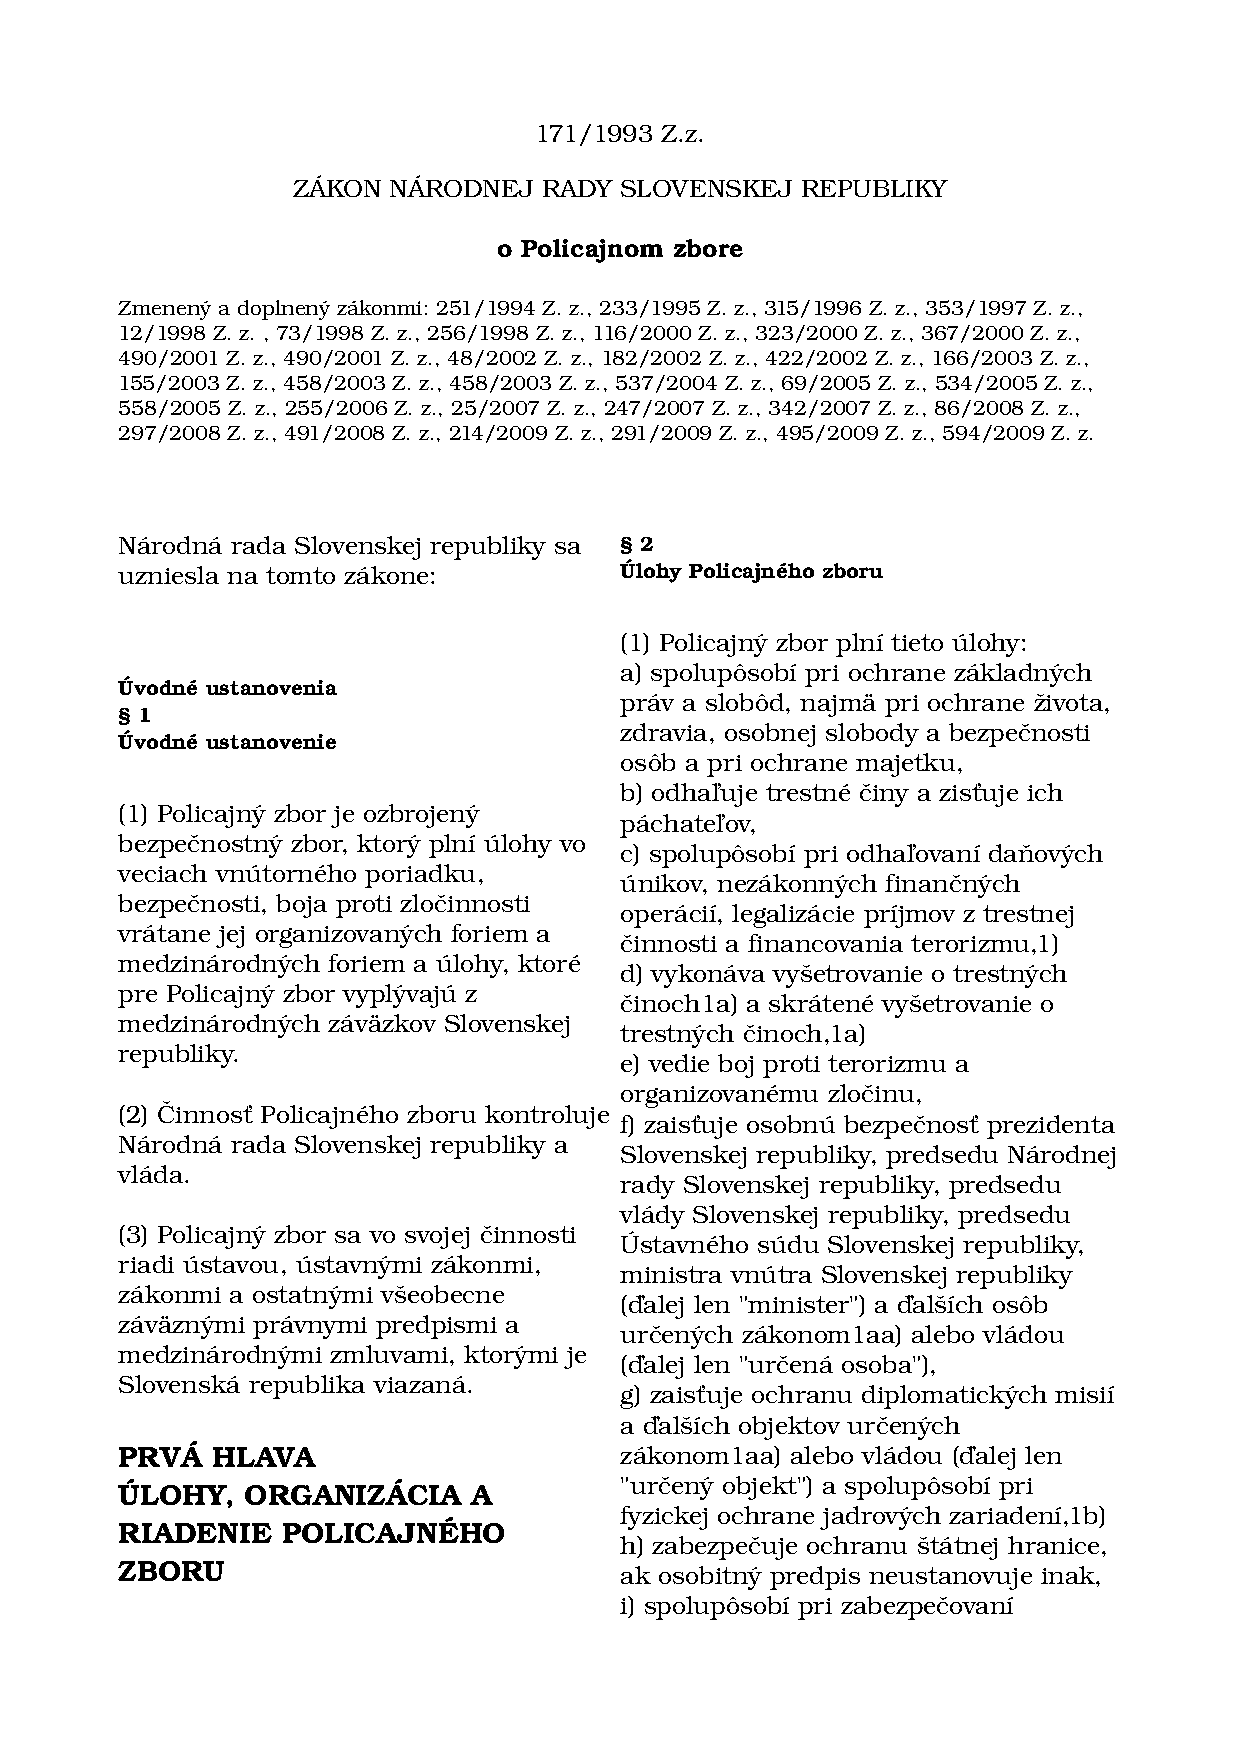
\includepdf[pages=-]{policia.pdf}
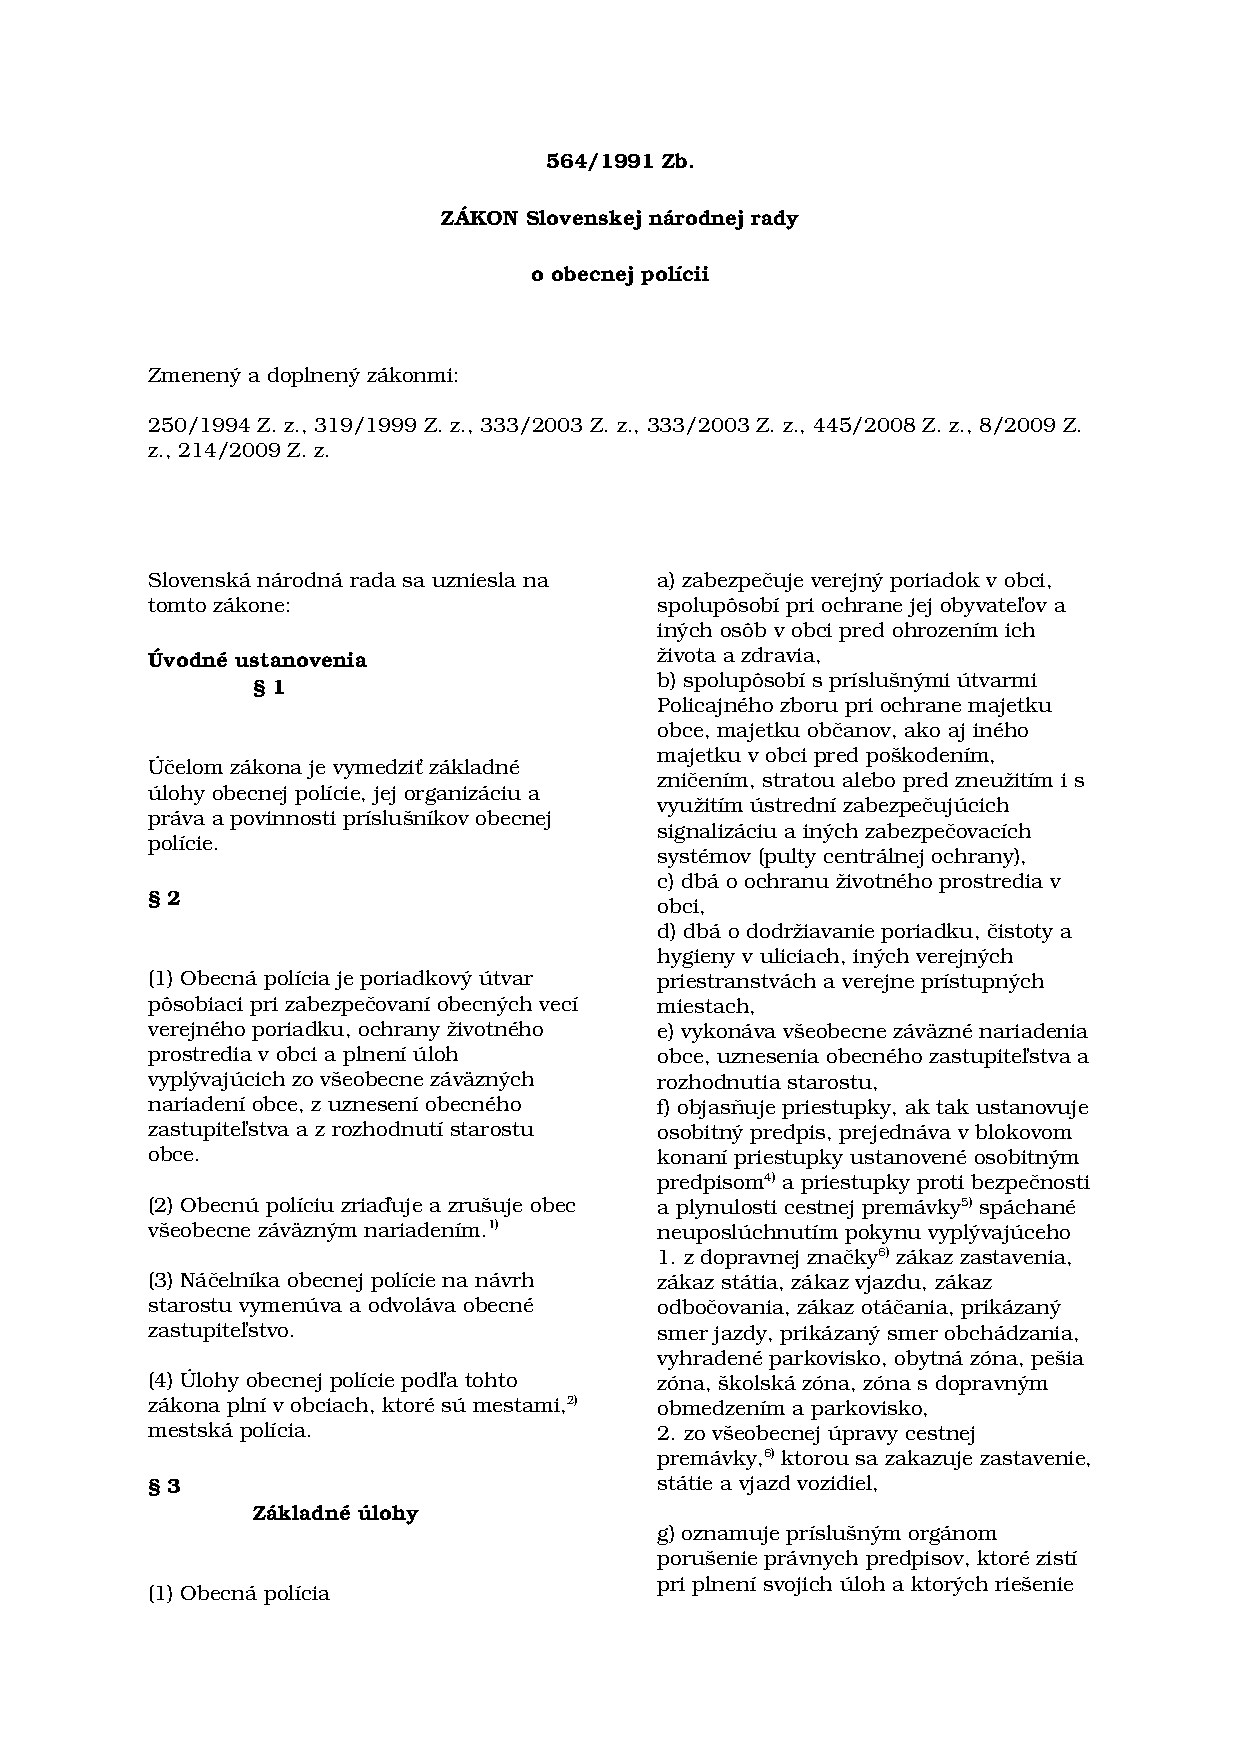
\includepdf[pages=-]{obecna.pdf}


\end{document}
